%% -*- mode: latex; mode: flyspell -*-
\documentclass[12pt, letter]{article}

%% Class name and Assignment number
%%
\newcommand{\courseName}{Introduction~to~Deep~Learning~for~Computer~Vision}
\newcommand{\assignName}{Assignment~7:~Convolutional~Neural~Networks~II}

%% Packages
\usepackage{amsmath,amsfonts,amssymb,amsthm,dsfont}
\usepackage{graphicx}
\usepackage[bookmarks=false]{hyperref}
\usepackage{color}
\usepackage{lipsum}

%% Paper format
\usepackage{geometry}
\geometry{
    letterpaper,
    %% total={216mm,279mm}, %< NSERC size
    margin=2.00cm,     %< default
    %% margin=1.87cm,       %< NSERC tightest
}

%% Headers and footers
\usepackage[explicit]{titlesec}
\newpagestyle{titlesec_assignment}{
  \sethead{\courseName}{}{\assignName}\setfoot{}{\thepage}{}
  \headrule
  %% \footrule
}

\begin{document}

%% Set header and footer
\pagestyle{titlesec_assignment}

%% Title
\title{\courseName\\\assignName}
\author{Paul Molina-Plant}

\maketitle

\abstract{In this assignment I completed the convolutional neural network
  implementation from the last assignement and improved the performance.}

\section{Reproducing default architecture results}

Following the assignment specification I finished the implementing the init,
conv, and forward pass of the model. Then I verified my testing results matched the expected accuracy of $62.68\%$.
\begin{figure}[!ht]
  \centering
  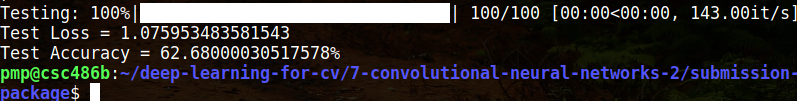
\includegraphics[width=0.8 \textwidth]{test.png}
  \caption{Testing on provided model.}
  \label{fig:test}
\end{figure}

\section{Debugging}
Too address the gpu-cpu issue, I added an argument to load the model onto the
appropriate computation device for the platform.
\begin{figure}[!ht]
  \centering
  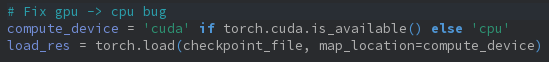
\includegraphics[width=0.8 \textwidth]{cpufix.png}
  \caption{Model loads correctly on cpu only platforms.}
  \label{fig:eg}
\end{figure}

\newpage

\section{Going beyond}
I tried many different architectures when attempting to improve the model's
accuracy on the test set. First I tried increasing the iterations, but this
plateaued at around $60\%$. Next I tried adding additional layers and neurons to
the network, this peaked around $66\%$. I tried the ReLU, Leaky ReLU, and ELU
activation functions, and found ELU provided the best results. Next I tried
increasing the learning rate and l2 regularization to reduce overfitting, this
peaked around $70\%$. Then I added additional input channels and increased the
size of the input convolutional layer. \\
My final model uses ELU for activation, 16 base channels, an outer convolutional
size of 5, a learning rate of $3e-3$, and an l2 regularization stength of
$1e-3$. The model was trained for 150 epochs. The final accuracy achived was
$74.5\%$. \\
When testing the model, please note the directory used for the saved
model is only ``save'' with no subdirectory.
\begin{figure}[!ht]
  \centering
  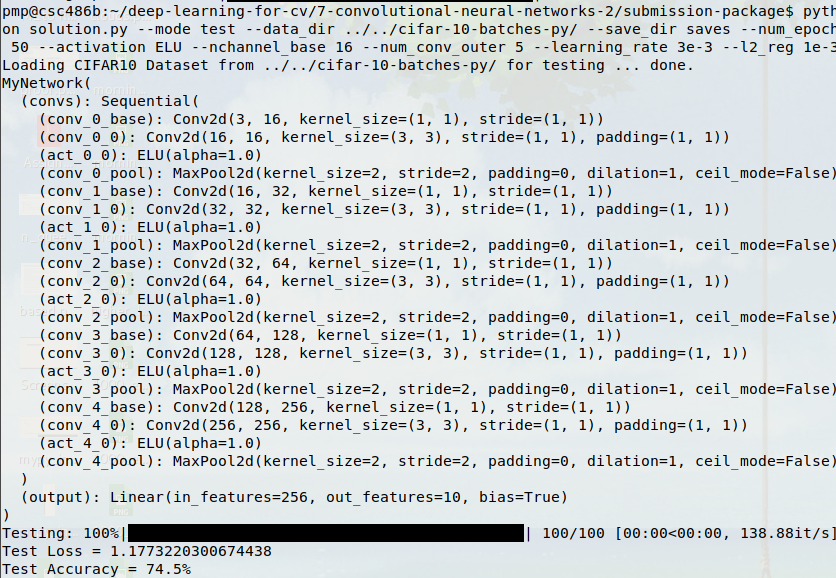
\includegraphics[width=0.8 \textwidth]{result.png}
  \caption{Model testing output.}
  \label{fig:eg}
\end{figure}
\begin{figure}[!ht]
  \centering
  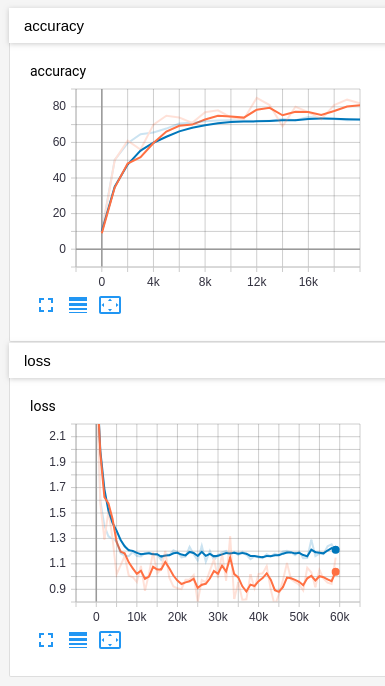
\includegraphics[width=0.6 \textwidth]{graph.png}
  \caption{Model training graphs.}
  \label{fig:eg}
\end{figure}

\end{document}

%%% Local Variables:
%%% mode: latex
%%% TeX-master: t
%%% End:
